
\documentclass{article}

%\usepackage{amsmath}
%\usepackage{apacite}
%\usepackage[pdftex]{graphicx}
\usepackage{graphicx}
\usepackage{mslapa}
\usepackage[section]{placeins}  % place a \FloatBarrier in each section
\usepackage{url}
\usepackage{fullpage}  % to standard 1 inch margins

\raggedright

\begin{document}
\setlength{\parindent}{1cm}

\title{Engine Tuning with Msqdev}
\author{Jeremiah Mahler}
\date{\today}

\maketitle

\tableofcontents

\pagebreak

\section{Introduction}

Tuning an engine can be easy or difficult depending upon
how many variables are available to be altered.
For example if ignition timing is controlled by a mechanical
distributor the only variable that can be changed is the base timing.
If it is computer controlled then there is an entire map
of variables that can be changed.

Megasquirt \cite{MEGA11} is an open source fuel injection and ignition
control system.
It provides a huge number variables that can be altered but
it is also difficult to optimize.

The Msqdev system \cite{MAHL11} was created to make
Megasquirt easier to optimize.
It controls the ecu through an interface of files and directories.
Tables are defined in a format which is easy to edit.
Programs are provided (or can be written) which can
collect data or modify settings in an automated manner.
And the data can be analyzed with a system such as R \cite{R}.

In general the goal of tuning is to find two points to compare
and to choose the best one.
Ideally all the variables in the two points to compare should be
the same except for the one variable that is varied.
Achieving this with Megasquirt can be difficult.
For example, to keep the ignition timing constant all the values in
the ignition map could be set to the same value.
But there are other settings, such as "MAT Based Timing Retard"
which are dependent on the ignition map and influence the timing.
There are even settings which when set to zero (which suggests they
would have no effect) actually do such as with the "Nonlinear MAT Correction".

The design of Msqdev consists of various parts.
The \verb+msqdev+ daemon establishes the interface between the files and the
Megasquirt ecu.
There are utilities such as \verb+msq-ve_tuner+ for automatically
tuning the fuel mixture and \verb+msq-accel_tuner+ for performing
acceleration tuning.
Plotting and analysis of captured data is most often done using
R \cite{R} scripts.
Small robust programs are preferred over large all encompassing
programs.

\section{Steady State Tuning}
\label{sec:steadytun}

Steady state tuning is done when the engine rpms are stable such as
at idle.
Its use under heavier load conditions is possible but it is difficult to
balance load exactly to the power output.

Steady state tuning is performed by altering variables and then measuring
the new steady state.
As an example consider varying the fuel mixture at idle to maximize rpm.
In a range around the current mixture each setting has a corresponding
rpm (see Figure \ref{fig:sstrpm}).
The setting closest to the maximum is the best setting.

% TODO - rebuild this as a pdf so it looks better
\begin{figure}[tbp]
\center
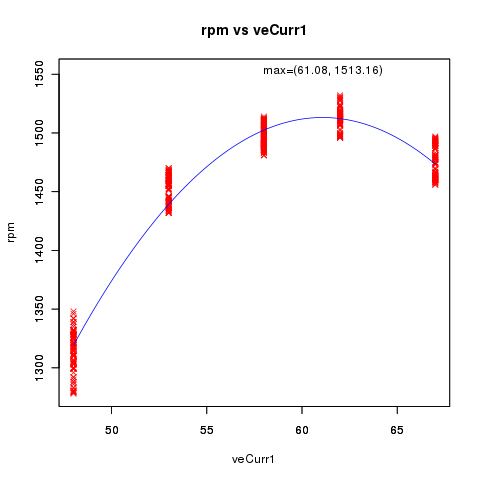
\includegraphics[scale=0.5]{plot01}
\caption{Steady State Tuning by varying veCurr1 vs rpm at idle.}
\label{fig:sstrpm}
\end{figure}

The order in which the variables are varied can be helpful in detecting
if there is any error caused by acceleration.
Suppose, for example that the engine rpms were decelerating.
If the variables were varied from one boundary to the other it would have
decreasing slope.
If instead the variables were varied from the center to one boundary and then
back to the center to the other boundary the center point will be
separated if there was any acceleration (Figure \ref{fig:ssrerr}).

% TODO - rebuild this as a pdf so it looks better
\begin{figure}[tbp]
\center
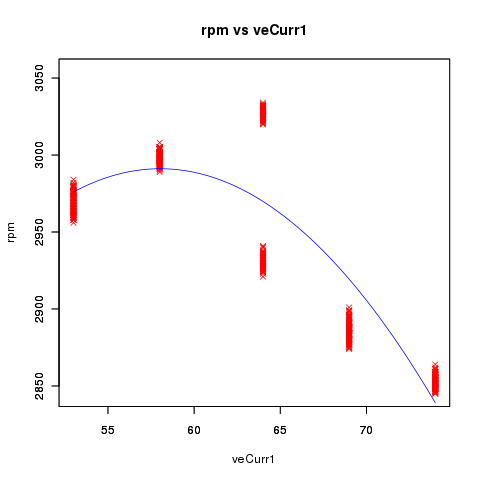
\includegraphics[scale=0.5]{plotdata-veTable1-20110613-15:17:10.png}
\caption{Steady state tuning with a large deceleration error
indicated by the gap in the center..}
\label{fig:ssrerr}
\end{figure}

\section{Acceleration Tuning}
\label{sec:acctun}

In contrast to Steady State Tuning (Section \ref{sec:steadytun}), Acceleration
Tuning is done when the engine rpms are increasing or decreasing.
This method is more useful than Steady State Tuning because it can be
applied to far more situations and does not depend on balanced conditions.

One source of error with acceleration tuning is with the throttle position.
A human operator is quite imprecise and can easily allow significant
throttle movement without their knowledge.
To reduce this error a throttle stop can be used.
The throttle stop is a fixed length object such as a piece of tubing which
can be placed underneath the gas pedal to limit its travel.
Support in the tuning program can provided to start/stop recording so
that a trial is only recording while the pedal is against the stop.

% TODO - picture of throttle stop

%This utility works by comparing two data recordings from two accelerations
%under the same conditions but with different settings.
%From the better setting the values will be shifted up/down and the process
%repeated.
%Eventually it will reach a maximum where it can no longer find a better
%set of settings and this will be the best.

\section{Air Fuel Ratio}
\label{sec:afr}

% good introduction
The fuel mixture is crucial in determining how well an engine runs.
If it is too rich or too lean the engine will lack power.
To minimize emissions the stoichiometric mixture is best.
To maximize power a richer than stoichiometric mixture is best.
To maximize fuel economy a leaner than stoichiometric mixture is best.
Obviously only one of these can be maximized at a time for a given
point on the map.
In general the goal of any of these is to achieve a specific fuel
mixture for specific operating conditions.

The desired air fuel ratio can be found by incrementally adjusting
values while the engine is running until the desired value is achieved.
This procedure also results in many data samples of settings and their
resulting air fuel ratios.
To go beyond merely achieving a single desired air fuel ratio, this data
can be used to build a function which predicts what the air
fuel ratio will be.
This has the added benefit of being able to instantly set the air fuel ratio
to any desired value.

\subsection{Predicting The Air Fuel Ratio}
\label{sec:predafr}

% procedure, step 1
The first step in building a function which can predict the air fuel ratio
is to record data.
This is accomplished in the Msqdev system using \verb+msq-ve_tuner+ utility.
This utility will attempt to adjust the current ve values to achieve
a specific air fuel ratio.
The engine should be run through various rpm ranges and various load values.
Whether the desired air fuel ratio is achieved is not important,
rather data samples of the air fuel ratio for a given setting are what
matter.

% procedure, step 2
Once a adequate data sample has been recorded it can be processed 
using the R script \verb+ve_tuner.R+ (Appendix \ref{app:vetuner})
which performs a least squares fit to find the coefficients which define
the linear function.
These coefficients can then be used with the Msqdev utility \verb+msq-afr_table+
to build tables with any desired air fuel ratio.

\FloatBarrier  % keep all the figures in this section

\subsection{Finding The Air Fuel Ratio For Max Power}
\label{sec:findafrpow}

Once the function which predicts the air fuel ratio has been found
(Section \ref{sec:predafr}) the values can be varied to find which
one produces the maximum power (maximum acceleration).
In the Msqdev system this is accomplished using the utility
\verb+msq-accel_tuner+ for performing acceleration tuning (Section \ref{sec:acctun}).

\appendix
\section{ve\_tuner.R}
\label{app:vetuner}

% The following text was generated by appA-ve_tuner.tex.php
% Sun, 03 Jul 2011 14:46:32 -0700

\begin{verbatim}

# This script is used to perform a least squares fit of the data
# related to veTable1 to find the function that predicts the
# air fuel ratio.

# To run this script start R and source this file
#
# bash$ R
# > source("ve_tuner.R")
# Loading required package: MASS
# 
# Call: rlm(formula = afr1 ~ veCurr1 + fuelload + rpm, maxit = 40)
# Residuals:
#     Min      1Q  Median      3Q     Max 
# -4.1269 -0.4980 -0.1448  0.5697  3.0852 
# 
# Coefficients:
#             Value    Std. Error t value 
# (Intercept)  17.9873   0.0925   194.3936
# veCurr1      -0.1399   0.0023   -61.2773
# fuelload      0.0525   0.0016    33.8201
# rpm           0.0004   0.0000    25.2164
# 
# Residual standard error: 0.7837 on 12986 degrees of freedom
# >

# Once the coefficients are found a table can be built using
# the command below (with different values).
#
# bash$ msq-afr_table -afr 16.5 -a -0.1399 -b 0.0525 -c 0.0004 -d 17.9873

# Choose the file with the recorded data from msq-ve_tuner
#f1 <- "20110626-ve_tuner/msq-ve_tuner-20110626-16:47:48" # ok
f1 <- "20110626-ve_tuner/msq-ve_tuner-20110626-16:59:22" # good
#f1 <- "20110626-ve_tuner/msq-ve_tuner-20110626-17:12:36"  # ok

d1 <- read.csv(file=f1, head=TRUE, sep=",")


# Filter the data to remove invalid extreme values.

# Remove invalid extreme air fuel ratios
filt0 <- d1$afr1 > 10 & d1$afr1 < 16

# remove invalid idle and deceleration values
filt0 <- filt0 & d1$tps > 1

# remove near idle rpms
filt0 <- filt0 & d1$rpm > 2600

veCurr1  <- d1$veCurr1[filt0]  	# x
afr1 	 <- d1$afr1[filt0]  	# y
fuelload <- d1$fuelload[filt0]  # z
rpm 	 <- d1$rpm[filt0]


# account for delay in afr1
#dX <- 0
#dX <- 10  # ok
dX <- 20  # ok
#dX <- 40
#dX <- 60  # too far
# shift forward
afr1 <- afr1[(dX + 1):length(afr1)]
# shift back
veCurr1 <- veCurr1[1:(length(veCurr1) - dX)]
fuelload <- fuelload[1:(length(fuelload) - dX)]
rpm <- rpm[1:(length(rpm) - dX)]

#lmfit1 <- lm(formula = afr1 ~ veCurr1 + fuelload + rpm)
require(MASS)  # rlm
lmfit1 <- rlm(formula = afr1 ~ veCurr1 + fuelload + rpm, maxit=40)

print(summary(lmfit1))


\end{verbatim}


\pagebreak

\bibliographystyle{mslapa}
%\bibliographystyle{plain}
%\bibliographystyle{acm}
%\bibliographystyle{ieeetr}
\bibliography{main}

\end{document}
